

\section{Experiments}\label{sec:experiments}
%
In this section, we evaluate the performance of our methods with our competitors on real data sets.
% We will conduct experiments
We have implemented two variants of our methods (SPC and SPC$^*$).
%for extracting statistics of queries, benchmarking the cost of a shortest path call,
%and selecting promising paths from a query log $\mathcal{QL}$ into the cache.
They share the same techniques in Section~\ref{sec:BenefitDriven},
and only differ in their cache structures:
(i) SPC uses a path array cache (Section~\ref{sec:cacheLookup}), and (ii) SPC$^*$ uses the compressed graph cache (Sections~\ref{sec:cacheSubgraph},\ref{sec:cacheCompress}).
%
Our competitors are LRU (a dynamic caching method) and HQF (a static caching method).
They have been introduced in Section~\ref{sec:competitors}.
All the above methods are written in C++.
We conduct our experiments on an Intel i7 3.4GHz PC running Debian.

%  (ii) SPC$^+$ uses a graph cache (Section~\ref{sec:cacheSubgraph}),
%SPC, our method, with the 3 cache representation schemes - List cache, Graph cache, Compressed Graph cache - described in section
{\color{red}
We will evaluate the above methods for a cache located at the proxy, and for a cache located at the server.
For the proxy scenario, the performance measure is the hit ratio.
For the server scenario, the performance measures are: (i) the percentage of running time saved on the server, compared to using no cache,
and (ii) the percentage of road network nodes visits saved, compared to using no cache.
}

%in both the proxy
%well both when considering the Proxy and Server scenario

%To compare how well we have done, we have implemented two baseline competitors, LRU and HQF. LRU is a dynamic caching method which evicts the Least recently used cache item if there is no space in the cache for new entries. HQF adds to the cache, the \spaths from the most frequent start-/end-points in the training data.





%Aalborg: total nodes in SPs from training set: 352032 in 1643 paths

%Beijing: total nodes in SPs from training set: 316400 in 6479 paths



%This is the most common usage of static caching in the web caching literature \cite{BaezaYates07}.


% In this section, we present the results of performance
% experiments, demonstrating the efficiency and real world applicability of the proposed algorithms. We


\subsection{Experimental Setting}
%
We are unable to obtain real query log from online shortest path services (e.g., Google Map), due to their privacy policies.
Thus, we can only simulate a query log from a trajectory data set.
For each trajectory, we extract its start location and its end location as the
source $v_s$ and destination $v_t$ of a shortest path query respectively.

We have used two real data sets, {\color{red} for their details see Table~\ref{tab:datasetsize}.
Each data set consists of (i) a collection of trajectories, which we use to simulate a query log}, and 
(ii) a corresponding road network for the trajectories.

%Which historical query data sets do we have, and what is their size and origin.

%- Aalborg: Query workload from and around the Danish city of Aalborg

%- Beijing: Query workload from Beijing



Following the experimental methodology of static caching~\cite{Ozcan2011},
we divide the query log into two equal sets.
The {\em historical query log} set is used for defining query frequencies and
for filling the cache content.
The {\em query workload set} set can only used for testing the performance of our method.


%We do not give a default size for the query-data sets Maps, as we will execute all of our tests, described in section \ref{subsec:expProxy} and \ref{subsec:expServer}, for each data set.


\begin{table}
\center
\begin{tabular}{|c|r|r|r|}\hline
Data set & $\#$ Trajectories / Queries & $\#$ Nodes & $\#$ Edges \\\hline
Aalborg & 4.401  & 129.680 & 137.470 \\\hline
Beijing & 12.928 & 76.226 & 85.882 \\\hline
\end{tabular}
\caption{Description of real data sets}
\label{tab:datasetsize}
\end{table}
%% Aalborg = Aalborg
%% Beijing = Beijing


%GPS trajectories

%according to XXX l

%The size of training and test query data sets are given already. The size of each data set, as well as the map they are captured on, is given in table \ref{tab:datasetsize}.



%% Aalborg = Aalborg
%% Beijing = Beijing


%We do not give a default size for the query-data sets Maps, as we will execute all of our tests, described in section \ref{subsec:expProxy} and \ref{subsec:expServer}, for each data set.




All caching methods, SPC, SPC*, HQF, and LRU, share a number of common settings which, unless stated otherwise, will be set to their default values:
The number of levels in the kD-tree is 14 (i.e. 16,384 regions). We will use the list cache representation as the default cache representation, where each vertex use one byte. The default cache size is set to 625 kB.

{\color{red} 
The default cache size, as well as the maximum cache size in later experiments (Fig.~\ref{fig:cSizeVsHitRatio}, \ref{fig:cacheSizeVsHitRuntime}, \ref{fig:cacheSizeVsNodesvisited}), is choosen baring in mind the size of the Aalborg and Beijing query logs. 
Had we had access to large data sets of real query logs, from online shortest path service providers, we would use a large cache size like 1 GB.}

% 
% 
% The size of our data sets is the limiting factor
% 

% 
% 
% \label{fig:cacheSizeVsHitRuntime}
% 
% \label{fig:cacheSizeVsNodesvisited}


% - Which parameters are common for all tests
% - What are the ranges/values each parameter can take.
% - Which parameters are set to a default value unless otherwise stated (and what are the default values)
% - Which methods, and in which configuration, do we consider.



\subsection{Caching in the Proxy Scenario}\label{subsec:expProxy}
%
In the proxy scenario, the shortest path call API would issue a shortest path query to the server,
rather than performing computation by itself (see Section~\ref{sec:benchmark}).
Since the total cost is dominated by the communication round-trip time with server,
we use the cache hit ratio as the performance measure in this scenario.
In the default case it takes 61.4 and 43.4 seconds, for the Beijing and Aalborg data set respectively, to fill the cache with SPC. For SPC$^*$ filling the takes 123.4 and 100.9 seconds for the Beijing and Aalborg data set.
%The fill time values for max cache size (8192 kB) are: SPC 175.3/102.5 sec and SPC$^*$ 175.4/100.4 sec. for the Beijing and Aalborg data sets respectively.

For both data sets we vary the cache size and kD-tree levels to show the impact on the cache hit ratio. We have implemented a number of optimizations to the cache storage (See sec. \ref{sec:CacheStruct}) and show their impact on the cache hit ratio.


\stitle{Effect of the kD-tree level}
%
In Figure~\ref{fig:levelVsHitRatio}, we vary the kD-tree level from 8 to 16 levels and show that using a kD-tree of about 14 levels can significantly increase the cache hit ratio of both the Aalborg and Beijing data set. SPC$^*$ performs better than SPC.


\begin{figure}[htb]
\center
  \begin{tabular}{@{}c@{ }c@{}}
     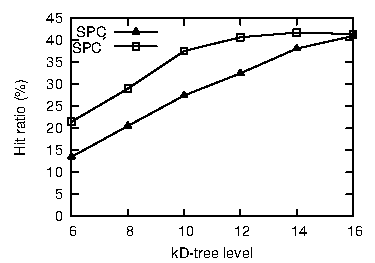
\includegraphics[width=0.5\columnwidth]{figures/split_hitratio_aal.pdf}
     &
     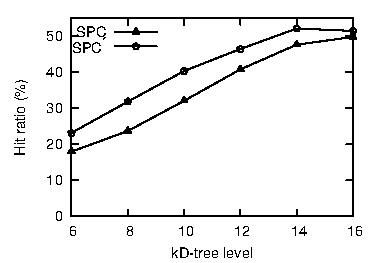
\includegraphics[width=0.5\columnwidth]{figures/split_hitratio_bei.pdf}
      \\
     (a) Aalborg & (b)  Beijing
     \end{tabular}
\caption{Hit ratio vs. Levels}
\label{fig:levelVsHitRatio}
\end{figure}

{\color{red}
On both data set SPC* outperforms SPC by 5-10\% in hit ratio. On both data sets SPC$^*$ performs 10\% better than SPC, up to level 12, in term of hit ratio. After level 12 SPC and SPC$^*$ start to converge toward the same hit ratio. Both data sets clearly show the benefit of using levels.
}



\stitle{Effect of the cache size}
%
In Figure~\ref{fig:cSizeVsHitRatio}, we measure the hit ratio of the methods
while varying the cache size from 1 kB to 5 MB.


\begin{figure}[htb]
\center
  \begin{tabular}{@{}c@{ }c@{}}
     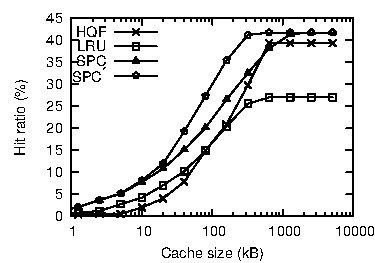
\includegraphics[width=0.5\columnwidth]{figures/cachesize_hitratio_aal.pdf}
     &
     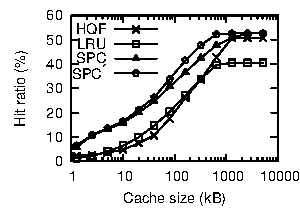
\includegraphics[width=0.5\columnwidth]{figures/cachesize_hitratio_bei.pdf}
      \\
     (a) Aalborg & (b)  Beijing
     \end{tabular}
\caption{Hit ratio vs. cache size}
\label{fig:cSizeVsHitRatio}
\end{figure}

{\color{red}



We can see that LRU consistently perform worse than SPC and SPC$^*$ for all cache sizes. The cache hit ratio stabilizes at about 26 and 40\% for Aalborg and Beijing respectively. Since LRU levels out at a much lower cache hit ratio than all of it's competitors it is not a suitable choice for \spath caching.

The performance of HQF is quite low at smaller cache sizes. While HQF can outperform LRU at larger cache sizes, it is consistently performing worse than SPC and SPC$^*$, making it a sub-optimal choice for \spath caching.

SPC and SPC$^*$ both outperform HQF and LRU for all sizes of the cache .Both SPC and SPC$^*$ have the same maximum cache hit ratio since they are using the same same caching scheme, with different representations of the cache. SPC$^*$ is the better choice of the two, as it performs as least as well, and often better, than SPC, for all cache sizes. 
}





\subsection{Caching in the Server Scenario}\label{subsec:expServer}
%
In the server scenario, the shortest path API has to invoke a shortest path algorithm.
{\color{red}
Thus, the relative savings running time, compared to not using a cache, is the most important performance measure. We also measure the relative saving in the number of nodes visited in a shortest path algorithm, which serves an indicator of the running time.
%On a server our aim is slightly different than on the Proxy, as we also have to consider that there may be some paths that are so small that it may be cheaper to simply re-calculate the result, instead of caching it.
%For the server scenario we will test the cache hit ratio, running time, and Nodes visited.
%For all three experiments
%We will vary kD-tree levels and cache size in the following experiments.
As a case study, we use the Dijkstra's and A$^*$ algorithms as the shortest path algorithm to show the benefit of using a \spath cache with different \spath algorithms.

In the following experiments, the query time saving ratio (and visited nodes saving ratio) refer to the running time saved (and nodes visited) when compared to not using any caching. 
The query time saving ratio is calculated as total time used to execute query workload without using caching $NC_t$ minus the total time to execute the query workload using caching $C_t$, divided by the total time to execute query workload without using caching times 100. The equation to compute the time saving ratio: $ \frac{NC_t - C_t}{NC_t}*100$.

Naming the total nodes visited by the shortest path algorithm without using caching as $NC_t$ and the total nodes visited by the shortest path algorithm using caching as $C_t$, we use the same equation to compute the visited nodes saving ratio.

The total query time and total nodes visited using when not using caching is presented in table \ref{tl:nonemethod}.

The results presented are for processing the entire query workload. The difference is presented as a ratio between using a caching scheme and using no caching scheme at all.
}




\begin{table}[htb]
\center
\begin{tabular}{|l|r|r|}\hline
 & Query time (sec.) & Nodes visited \\\hline \hline
Aalborg - Dijkstra & 18.50 & 18580659 \\\hline
Beijing - Dijkstra & 43.50 & 41615917 \\\hline
Aalborg - A$^*$ & 4.5 & 2929128 \\\hline 
Beijing - A$^*$ & 9.8 & 6544620 \\\hline
\end{tabular}
\caption{Query time and nodes visited, not using caching}
\label{tbl:nonemethod}
\end{table}



\stitle{Estimation of shortest path running cost}
{\color{blue} Do the table and its explanation need to be updated since we have updated both approach, workload, and map data?}

First, we test the estimation error of our cost estimation technique proposed in Section~\ref{sec:benchmark}.
We measure the error percentage in terms of the relative error between the actual cost and the estimated cost.
Table~\ref{tbl:estcost} shows the estimation error of our technique
as a function of: (a) the number of landmark $|U|$, and (b) the size of the samples $S$.
The default values are: $|U|=20$ and $S=100$.
The majority of errors are below 30\% and thus our estimation technique is reasonably accurate.


%% Aalborg: average cost = 136347/2 = 68173
%%  Beijing: average cost = 79603/2 = 39801
%  average because random node chosen



\begin{table}
\center
\color{blue}
\begin{tabular}{cc}
    \begin{tabular}{|c|c|c|}
    \hline
    $|U|$ & Aalborg & Beijing \\ \hline \hline
     5 & 35.5 & 33.3 \\ \hline
     10 & 25.4 & 28.2 \\ \hline
     20 & 22.2 & 23.9 \\ \hline
     40 & 19.4 & 23.0  \\ \hline
     80 & 19.9 & 21.9 \\ \hline
    \end{tabular}
    &
    \begin{tabular}{|c|c|c|}
    \hline
    $S$ & Aalborg & Beijing \\ \hline \hline
     25 & 23.4 & 28.8 \\ \hline
     50 & 20.7 & 28.4 \\ \hline
     100 & 22.2 & 23.9 \\ \hline
     200 & 20.4 & 22.7 \\ \hline
     400 & 21.1 & 21.3 \\ \hline
    \end{tabular}
    \\
    (a) varying number of landmark $|U|$ & (b) varying sample size $S$
\end{tabular}
    \caption{Average error percentage of cost estimation}
    \label{tbl:estcost}
\end{table}








%
\stitle{Effect of the kD-tree level}
%
{\color{red}
In Figure~\ref{fig:split_diffnodes_server}, \ref{fig:split_diffruntime_server}, \ref{fig:split_diffnodes_server_astar}, \ref{fig:split_diffruntime_server_astar}, we again vary the kD-tree level from 6 to 16 levels. 

All four experiments shows a consistent advantage of using SPC$^*$ over SPC. 


Figure \ref{fig:split_diffnodes_server}/\ref{fig:split_diffruntime_server} shows the performance SPC and SPC$^*$ using the Dijkstra \spath algorithm.

In figure \ref{fig:split_diffnodes_server}a and b we can see that SPC and SPC$^*$ performs very stable, achieving almost the same saving in nodes visited on both the Aalborg and Beijing data set. SPC provides up to a 26\% saving in nodes visited, and SPC$^*$ gets up to a 30\% saving of nodes visited on the Beijing data set.

In figure \ref{fig:split_diffruntime_server}a and b we can see that increasing the levels provide significant run time savings for both SPC and SPC$^*$.
SPC does well, saving up to 15\% in running time, while SPC$^*$ achieves up to a 34\% reduction in running time. Both SPC and SPC$^*$ has a very stable performance. The time saved increases in all cases with more regions.


Figure \ref{fig:split_diffnodes_server_astar}/\ref{fig:split_diffruntime_server_astar} shows the performance SPC and SPC$^*$ using the A$^*$ \spath algorithm.

In figure \ref{fig:split_diffnodes_server_astar}a and b we can see that SPC and SPC$^*$ performs very stable, achieving performance very similar to using Dijkstra (see fig. \ref{fig:split_diffnodes_server}).


In figure \ref{fig:split_diffruntime_server_astar}a and b we can see that A$^*$s faster performance excludes SPC as a candidate, as it at its best still is about 18\% slower than not using any caching. Except for kD-tree level of 6 on the Aalborg data set, we can see that SPC$^*$ is very fast at answering the query workload as using it will consistently provide a time saving of 5-30\%. The time saved increases in all cases with more regions/ higher levels.

}



\begin{figure}[htb]
\center
  \begin{tabular}{@{}c@{ }c@{}}
     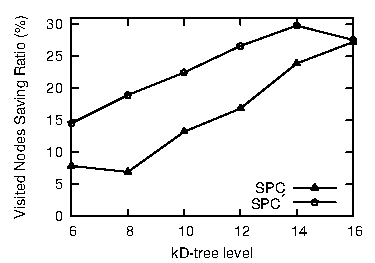
\includegraphics[width=0.5\columnwidth]{figures/split_diffnodes_aal_server.pdf}
     &
     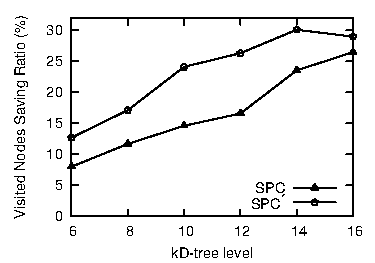
\includegraphics[width=0.5\columnwidth]{figures/split_diffnodes_bei_server.pdf}
      \\
     (a) Aalborg & (b)  Beijing
     \end{tabular}
\caption{Node Visits Saved vs. Levels using Dijkstra}
\label{fig:split_diffnodes_server}
\end{figure}


\begin{figure}[htb]
\center
  \begin{tabular}{@{}c@{ }c@{}}
     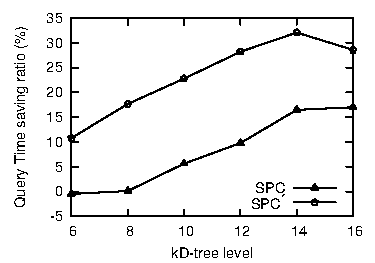
\includegraphics[width=0.5\columnwidth]{figures/split_diffruntime_aal_server.pdf}
     &
     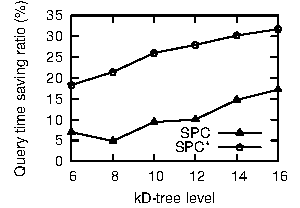
\includegraphics[width=0.5\columnwidth]{figures/split_diffruntime_bei_server.pdf}
      \\
     (a) Aalborg & (b)  Beijing
     \end{tabular}
\caption{Runtime Saved vs. Levels using Dijkstra}
\label{fig:split_diffruntime_server}
\end{figure}


\begin{figure}[htb]
\center
  \begin{tabular}{@{}c@{ }c@{}}
     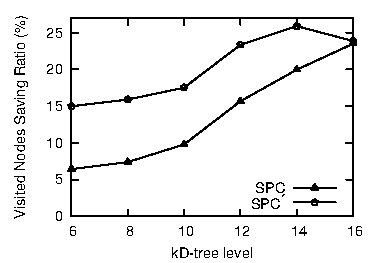
\includegraphics[width=0.5\columnwidth]{figures/split_diffnodes_aal_server_astar.pdf}
     &
     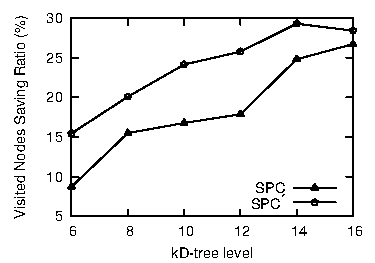
\includegraphics[width=0.5\columnwidth]{figures/split_diffnodes_bei_server_astar.pdf}
      \\
     (a) Aalborg & (b)  Beijing
     \end{tabular}
\caption{Node Visits Saved vs. Levels  using $A^*$}
\label{fig:split_diffnodes_server_astar}
\end{figure}



\begin{figure}[htb]
\center
  \begin{tabular}{@{}c@{ }c@{}}
     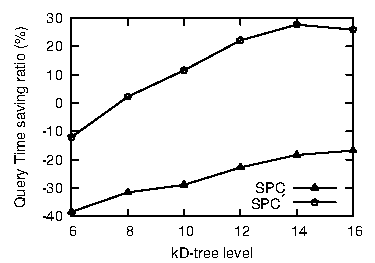
\includegraphics[width=0.5\columnwidth]{figures/split_diffruntime_aal_server_astar.pdf}
     &
     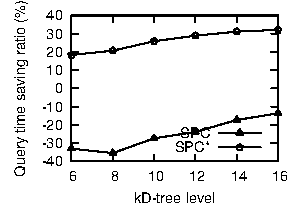
\includegraphics[width=0.5\columnwidth]{figures/split_diffruntime_bei_server_astar.pdf}
      \\
     (a) Aalborg & (b)  Beijing
     \end{tabular}
\caption{Runtime Saved vs. Levels using $A^*$}
\label{fig:split_diffruntime_server_astar}
\end{figure}





\stitle{Effect of the cache size}
{\color{red}
In the following experiments, we vary the cache size and observe the effect on visited nodes saved ratio and the query time saving ratio.




Figure \ref{fig:cachesize_diffnodes_server}/\ref{fig:cachesize_diffruntime_server} shows the performance SPC and  using the Dijkstra \spath algorithm.

In figure \ref{fig:cachesize_diffnodes_server}a and b we can see that LRU consistently perform worse than SPC and SPC$^*$ for all cache sizes. For both the Aalborg and Beijing data set LRU stabilizes at a visited nodes saving ratio of 20\%, about 2/3 of its competitors. 
For lower cache sizes SPC$^*$ outperforms all it its competitors. At larger cache sizes of a MB and above, HQF, SPC and SPC$^*$ all have the same visited nodes saving ratio of about 28\%.

In figure \ref{fig:cachesize_diffruntime_server}a we can see that as the cache size increases all caching schemes save more query time. Compared to its competitors SPC$^*$ performs significantly better, with a query time saving ratio of almost twice that of all its competitors. 
In figure \ref{fig:cachesize_diffruntime_server}b we can see that HQF, LRU, and SPC all perform poorly with a query time saving ratio of 0-5\%. SPC$^*$ performs consistently well and achieves a query time saving ratio above 30\%.


Figure \ref{fig:cachesize_diffnodes_server_astar}/\ref{fig:cachesize_diffruntime_server_astar} shows the performance SPC and SPC$^*$ using the A$^*$ \spath algorithm.

In figure \ref{fig:cachesize_diffnodes_server_astar}a and b we can see that SPC and SPC$^*$ performs very stable, achiving performance very similar to using Dijkstra (see fig. \ref{fig:cachesize_diffnodes_server}).

In figure \ref{fig:cachesize_diffruntime_server_astar}a and b we can see a very similar behaviour in both graphs. It is clear that neither HQF, LRU, or SPC are viable caching schemes when using the A$^*$ in the server scenario. All 3 caching schemes adds significt added running time, up to 90\% extra time on the Beijing data set.
}




\begin{figure}[htb]
\center
  \begin{tabular}{@{}c@{ }c@{}}
     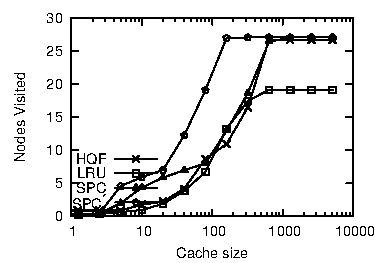
\includegraphics[width=0.5\columnwidth]{figures/cachesize_diffnodes_aal_server.pdf}
     &
     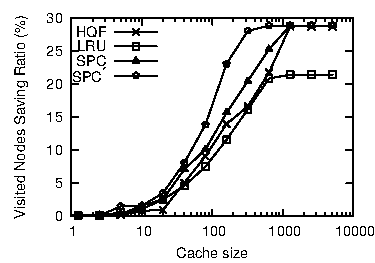
\includegraphics[width=0.5\columnwidth]{figures/cachesize_diffnodes_bei_server.pdf}
      \\
     (a) Aalborg & (b)  Beijing
     \end{tabular}
\caption{Node Visits Saved vs. Cache Size using Dijkstra}
\label{fig:cachesize_diffnodes_server}
\end{figure}

\begin{figure}[htb]
\center
  \begin{tabular}{@{}c@{ }c@{}}
     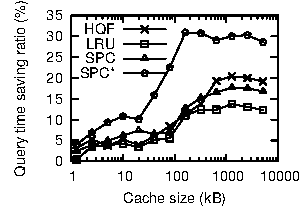
\includegraphics[width=0.5\columnwidth]{figures/cachesize_diffruntime_aal_server.pdf}
     &
     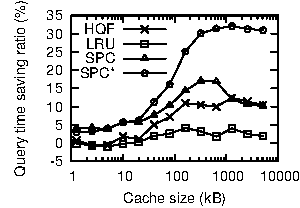
\includegraphics[width=0.5\columnwidth]{figures/cachesize_diffruntime_bei_server.pdf}
      \\
     (a) Aalborg & (b)  Beijing
     \end{tabular}
\caption{Runtime Saved vs. Cache Size using Dijkstra}
\label{fig:cachesize_diffruntime_server}
\end{figure}

\begin{figure}[htb]
\center
  \begin{tabular}{@{}c@{ }c@{}}
     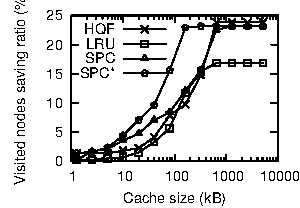
\includegraphics[width=0.5\columnwidth]{figures/cachesize_diffnodes_aal_server_astar.pdf}
     &
     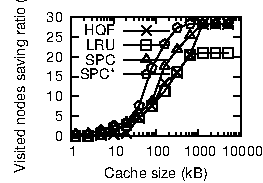
\includegraphics[width=0.5\columnwidth]{figures/cachesize_diffnodes_bei_server_astar.pdf}
      \\
     (a) Aalborg & (b)  Beijing
     \end{tabular}
\caption{Node Visits Saved vs. Cache Size using $A^*$}
\label{fig:cachesize_diffnodes_server_astar}
\end{figure}


\begin{figure}[htb]
\center
  \begin{tabular}{@{}c@{ }c@{}}
     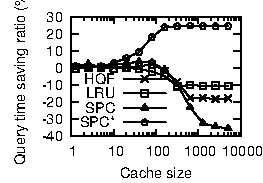
\includegraphics[width=0.5\columnwidth]{figures/cachesize_diffruntime_aal_server_astar.pdf}
     &
     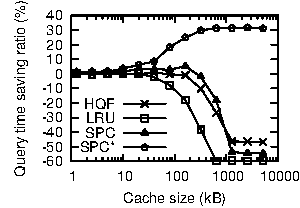
\includegraphics[width=0.5\columnwidth]{figures/cachesize_diffruntime_bei_server_astar.pdf}
      \\
     (a) Aalborg & (b)  Beijing
     \end{tabular}
\caption{Runtime Saved vs. Cache Size using $A^*$}
\label{fig:cachesize_diffruntime_server_astar}
\end{figure}





